% Khung ban đầu do P1 tạo; P6 phụ trách ghép và hoàn thiện slide.
% Biên dịch bằng XeLaTeX từ thư mục slides.
\documentclass[aspectratio=169,11pt]{beamer}
\usepackage{fontspec}
\setsansfont{texgyreheros}[Extension=.otf,UprightFont=*-regular,
  BoldFont=*-bold,ItalicFont=*-italic,BoldItalicFont=*-bolditalic]
\setmainfont{texgyretermes}[Extension=.otf,UprightFont=*-regular,
  BoldFont=*-bold,ItalicFont=*-italic,BoldItalicFont=*-bolditalic]
\setmonofont{texgyrecursor}[Extension=.otf,UprightFont=*-regular,
  BoldFont=*-bold,ItalicFont=*-italic,BoldItalicFont=*-bolditalic]
\usepackage[vietnamese]{babel}
\usepackage{amsmath,amssymb,booktabs}
\usepackage{tikz}
\usetikzlibrary{arrows.meta,positioning,shapes.geometric,calc}
\usetheme{Madrid}
\setbeamertemplate{navigation symbols}{}
\title[DFT -- ATPG]{Automatic Test Pattern Generation Algorithms for Combinational and Sequential Circuits}
\author[Nhóm 4]{Nhóm 4\\[3pt]
  {\footnotesize
  \begin{tabular}{@{}l@{\hspace{0.8em}}l@{\hspace{2.5em}}l@{\hspace{0.8em}}l@{}}
  Phan Ngọc Tuấn Nguyên & 23119178 & Phạm Trọng An Nam & 23119174\\
  Hà Quang Huy & 23119147 & Nguyễn Thị Thúy Hằng & 23119142\\
  Võ Trung Nguyên & 23119180 & Nguyễn Thị Thanh Tuyền & 23119222\\
  \end{tabular}}}
\institute[HCMUTE]{\footnotesize Trường Đại học Công nghệ Kỹ thuật TP. Hồ Chí Minh\\
  Khoa Điện -- Điện tử, Bộ môn Kỹ thuật Máy tính\\
  GVHD: Nguyễn Văn Thành Lộc}
\date{Tháng 10 năm 2026}
\begin{document}
\begin{frame}
\titlepage
\end{frame}
\begin{frame}{Vì sao cần testing và ATPG?}
\begin{itemize}
\item Verification: thiết kế có đúng đặc tả? Testing: chip chế tạo có lỗi?
\item Stuck-at: một dây bị kẹt 0 (SA0) hoặc 1 (SA1).
\item ATPG tìm mẫu làm đáp ứng mạch tốt khác mạch lỗi tại ngõ ra.
\end{itemize}
\begin{block}{Hai điều kiện bắt buộc}
Kích hoạt lỗi tại vị trí lỗi và lan truyền khác biệt đến ngõ ra quan sát được.
\end{block}
\end{frame}

% Sơ đồ c17 dùng cho slide 3 (chỉ số hiệu dây) và slide 4 (có giá trị, đường lỗi đỏ).
\newif\ifPOneVal
\newcommand{\POneLab}[2]{\ifPOneVal #2\else #1\fi}
\newcommand{\POneCseventeen}{%
\begin{tikzpicture}[x=1cm,y=0.85cm,line width=0.7pt,
 every node/.style={font=\ifPOneVal\large\else\small\fi},
 nand/.pic={
 \draw (-0.45,-0.4)--(-0.45,0.4)--(0,0.4)
 arc[start angle=90,end angle=-90,radius=0.4]--cycle;
 \draw (0.46,0) circle[radius=0.06];
 \coordinate (-a) at (-0.45,0.22);
 \coordinate (-b) at (-0.45,-0.22);
 \coordinate (-out) at (0.52,0);}]
\ifPOneVal\tikzset{lp/.style={red!75!black,very thick},lc/.style={red!75!black}}%
\else\tikzset{lp/.style={},lc/.style={}}\fi
\pic (g10) at (2.5,4) {nand};
\pic (g11) at (2.5,2.5) {nand};
\pic (g16) at (6,1.9) {nand};
\pic (g19) at (6,0) {nand};
\pic (g22) at (9,3.6) {nand};
\pic (g23) at (9,0.7) {nand};
\foreach \id/\x/\y in {10/2.5/4,11/2.5/2.5,16/6/1.9,19/6/0,22/9/3.6,23/9/0.7}
 \node[font=\footnotesize] at (\x,\y) {N\id};
\node[left] at (0,4.22) {\POneLab{1}{$1=X$}};
\node[left] at (0,3.25) {\POneLab{3}{$3=0$}};
\node[left] at (0,2.28) {\POneLab{6}{$6=X$}};
\node[left] at (0,1.4) {\POneLab{2}{$2=1$}};
\node[left] at (0,-0.22) {\POneLab{7}{$7=X$}};
\draw (0,4.22)--(g10-a);
\draw (0,3.25)--(1.3,3.25);
\draw (1.3,3.25)|-(g10-b);
\draw (1.3,3.25)|-(g11-a);
\fill (1.3,3.25) circle[radius=0.035];
\draw (0,2.28)--(g11-b);
\draw (0,1.4)--(4.9,1.4)|-(g16-a);
\draw (0,-0.22)--(g19-b);
\draw (g10-out)--(7.8,4)|-(g22-a);
\node[above] at (5.2,4) {\POneLab{10}{$10=1$}};
\draw[lp] (g11-out)--(3.9,2.5)--(3.9,1.68)--(g16-b);
\draw (3.9,1.68)|-(g19-a);
\fill[lc] (3.9,1.68) circle[radius=0.045];
\node[above,lc] at (4.25,2.5) {\POneLab{11}{$11=D$}};
\node[below,font=\scriptsize,red!75!black] at (3.35,2.5) {SA0};
\draw[red!75!black,thick] (3.25,2.42)--(3.41,2.58) (3.25,2.58)--(3.41,2.42);
\draw[lp] (g16-out)--(7.15,1.9)|-(g22-b);
\draw (7.15,1.9)|-(g23-a);
\fill[lc] (7.15,1.9) circle[radius=0.045];
\node[left,lc] at (7.15,2.7) {\POneLab{16}{$16=D'$}};
\draw (g19-out)--(7.6,0)|-(g23-b);
\node[below] at (7.1,0) {\POneLab{19}{$19=X$}};
\draw[lp] (g22-out)--(10.3,3.6);
\node[right,lc] at (10.3,3.6) {\POneLab{22}{$22=D$}};
\draw (g23-out)--(10.3,0.7);
\node[right] at (10.3,0.7) {\POneLab{23}{$23=X$}};
\end{tikzpicture}}

\begin{frame}{Mạch ví dụ chung: c17 và lỗi 11/SA0}
\centering
\POneValfalse
\resizebox{0.86\textwidth}{!}{\POneCseventeen}
\par\medskip
\small 6 cổng NAND; 5 ngõ vào $1,2,3,6,7$; 2 ngõ ra $22,23$.
Lỗi cần tìm: \textcolor{red!75!black}{net 11 kẹt ở 0}.
\end{frame}

\begin{frame}{Kích hoạt và lan truyền lỗi 11/SA0}
\begin{columns}[c,onlytextwidth]
\column{0.57\textwidth}
\centering
\POneValtrue
\resizebox{\linewidth}{!}{\POneCseventeen}
\column{0.41\textwidth}
\footnotesize
\begin{enumerate}
\item \textbf{Kích hoạt:} đặt $3=0$ \(\Rightarrow\) $11=\overline{3\cdot6}$:
 tốt 1, lỗi 0, tức $11=D$.
\item \textbf{Lan truyền:} đặt $2=1$ \(\Rightarrow\)
 $16=\overline{2\cdot11}=D'$; đồng thời $10=\overline{1\cdot3}=1$.
\item $22=\overline{10\cdot16}=D$: \textbf{quan sát được lỗi} ở ngõ ra.
\end{enumerate}
\begin{block}{Mẫu theo thứ tự PI $(1,2,3,6,7)$}
$(X,1,0,X,X)$; điền $X=0$ được $01000$.
\end{block}
\end{columns}
\end{frame}

\begin{frame}{Lộ trình và tiêu chí kiểm chứng}
\begin{itemize}
\item D-algorithm và PODEM; cùng minh họa lỗi c17 11/SA0.
\item ATPG tuần tự: trạng thái, full scan và trải khung thời gian.
\item Cài đặt, trace, mô phỏng lỗi và coverage.
\item Coverage phải ghi rõ danh sách lỗi; hết giới hạn tìm kiếm là
\texttt{ABORTED}, không kết luận \texttt{UNTESTABLE}.
\end{itemize}
\begin{block}{Bài tập trong giáo trình (video 2--3 phút)}
Ví dụ Hình 4.5: $f=xy+\overline y z$, tìm mẫu cho $y/SA0$.
\end{block}
\end{frame}

\begin{frame}{D-calculus: quan sát mạch tốt và mạch lỗi}
\centering
\begin{tabular}{c|cc}
Giá trị & Tốt & Lỗi\\\hline
$0$ & 0 & 0\\
$1$ & 1 & 1\\
$X$ & ? & ?\\
$D$ & 1 & 0\\
$\overline D$ & 0 & 1
\end{tabular}
\begin{block}{Tính cổng trên từng thành phần}
$D\land1=D$, $D\land\overline D=0$, $D\land X=X$.\\
Qua NAND với ngõ vào phụ bằng 1: $D\leftrightarrow\overline D$.
\end{block}
\end{frame}

\begin{frame}{Bảng logic năm giá trị cho tám loại cổng}
\centering\scriptsize
\renewcommand{\arraystretch}{1.05}
\setlength{\tabcolsep}{3pt}
\begin{minipage}[t]{0.24\textwidth}\centering
\textbf{AND}\\[1pt]
\begin{tabular}{@{}c|ccccc@{}}
$a\backslash b$ & 0 & 1 & $X$ & $D$ & $\overline{D}$\\\hline
0 & 0 & 0 & 0 & 0 & 0\\
1 & 0 & 1 & $X$ & $D$ & $\overline{D}$\\
$X$ & 0 & $X$ & $X$ & $X$ & $X$\\
$D$ & 0 & $D$ & $X$ & $D$ & 0\\
$\overline{D}$ & 0 & $\overline{D}$ & $X$ & 0 & $\overline{D}$\\
\end{tabular}
\end{minipage}\hfill
\begin{minipage}[t]{0.24\textwidth}\centering
\textbf{NAND}\\[1pt]
\begin{tabular}{@{}c|ccccc@{}}
$a\backslash b$ & 0 & 1 & $X$ & $D$ & $\overline{D}$\\\hline
0 & 1 & 1 & 1 & 1 & 1\\
1 & 1 & 0 & $X$ & $\overline{D}$ & $D$\\
$X$ & 1 & $X$ & $X$ & $X$ & $X$\\
$D$ & 1 & $\overline{D}$ & $X$ & $\overline{D}$ & 1\\
$\overline{D}$ & 1 & $D$ & $X$ & 1 & $D$\\
\end{tabular}
\end{minipage}\hfill
\begin{minipage}[t]{0.24\textwidth}\centering
\textbf{OR}\\[1pt]
\begin{tabular}{@{}c|ccccc@{}}
$a\backslash b$ & 0 & 1 & $X$ & $D$ & $\overline{D}$\\\hline
0 & 0 & 1 & $X$ & $D$ & $\overline{D}$\\
1 & 1 & 1 & 1 & 1 & 1\\
$X$ & $X$ & 1 & $X$ & $X$ & $X$\\
$D$ & $D$ & 1 & $X$ & $D$ & 1\\
$\overline{D}$ & $\overline{D}$ & 1 & $X$ & 1 & $\overline{D}$\\
\end{tabular}
\end{minipage}\hfill
\begin{minipage}[t]{0.24\textwidth}\centering
\textbf{NOR}\\[1pt]
\begin{tabular}{@{}c|ccccc@{}}
$a\backslash b$ & 0 & 1 & $X$ & $D$ & $\overline{D}$\\\hline
0 & 1 & 0 & $X$ & $\overline{D}$ & $D$\\
1 & 0 & 0 & 0 & 0 & 0\\
$X$ & $X$ & 0 & $X$ & $X$ & $X$\\
$D$ & $\overline{D}$ & 0 & $X$ & $\overline{D}$ & 0\\
$\overline{D}$ & $D$ & 0 & $X$ & 0 & $D$\\
\end{tabular}
\end{minipage}

\vspace{3mm}
\begin{minipage}[t]{0.24\textwidth}\centering
\textbf{XOR}\\[1pt]
\begin{tabular}{@{}c|ccccc@{}}
$a\backslash b$ & 0 & 1 & $X$ & $D$ & $\overline{D}$\\\hline
0 & 0 & 1 & $X$ & $D$ & $\overline{D}$\\
1 & 1 & 0 & $X$ & $\overline{D}$ & $D$\\
$X$ & $X$ & $X$ & $X$ & $X$ & $X$\\
$D$ & $D$ & $\overline{D}$ & $X$ & 0 & 1\\
$\overline{D}$ & $\overline{D}$ & $D$ & $X$ & 1 & 0\\
\end{tabular}
\end{minipage}\hfill
\begin{minipage}[t]{0.24\textwidth}\centering
\textbf{XNOR}\\[1pt]
\begin{tabular}{@{}c|ccccc@{}}
$a\backslash b$ & 0 & 1 & $X$ & $D$ & $\overline{D}$\\\hline
0 & 1 & 0 & $X$ & $\overline{D}$ & $D$\\
1 & 0 & 1 & $X$ & $D$ & $\overline{D}$\\
$X$ & $X$ & $X$ & $X$ & $X$ & $X$\\
$D$ & $\overline{D}$ & $D$ & $X$ & 1 & 0\\
$\overline{D}$ & $D$ & $\overline{D}$ & $X$ & 0 & 1\\
\end{tabular}
\end{minipage}\hfill
\begin{minipage}[t]{0.46\textwidth}\centering
\textbf{NOT}\\[1pt]
\begin{tabular}{@{}c|ccccc@{}}
vào & 0 & 1 & $X$ & $D$ & $\overline{D}$\\\hline
ra & 1 & 0 & $X$ & $\overline{D}$ & $D$\\
\end{tabular}
\\[4mm]
\textbf{BUFF}\\[1pt]
\begin{tabular}{@{}c|ccccc@{}}
vào & 0 & 1 & $X$ & $D$ & $\overline{D}$\\\hline
ra & 0 & 1 & $X$ & $D$ & $\overline{D}$\\
\end{tabular}
\end{minipage}

\vspace{2mm}
{\footnotesize Hàng: ngõ vào $a$; cột: ngõ vào $b$. Dùng làm dữ liệu kiểm thử chung, khớp chương trình 160/160 ô.}
\end{frame}

\begin{frame}{D-algorithm: chọn cube, lan truyền và justify}
\begin{itemize}
\item NAND $(a,b,z)$: cover $(0,X,1)$, $(X,0,1)$, $(1,1,0)$.
\item PDCF cho $z/SA0$: $(0,X,D)$ hoặc $(X,0,D)$.
\item PDC: $(D,1,\overline D)$; ngõ vào phụ bằng 1 cho sai khác đi qua.
\item Giao cube: $X\cap v=v$; yêu cầu xác định trái nhau gây xung đột.
\item D-frontier: đầu vào có sai khác, đầu ra còn $X$.
\item J-frontier: đầu ra đã gán, đầu vào chưa justify được.
\end{itemize}
\begin{block}{Điều kiện thành công}
Sai khác tới PO, mọi yêu cầu được justify và nhất quán.\\
Xung đột: quay lui, khôi phục trạng thái và thử cube khác.
\end{block}
\end{frame}

\begin{frame}{c17, 11/SA0: lan truyền và justification}
\centering
\begingroup
\def\pTwoCSeventeenWidth{0.86\linewidth}
% P2: tái sử dụng hình mach_c17.jpg do người dùng cung cấp, không vẽ lại.
% Wrapper dùng được từ report/main.tex và slides/main.tex.
% Hình thể hiện cube tổng quát hóa (X,1,0,X,X).
\IfFileExists{figures/common/mach_c17.jpg}{%
  \includegraphics[width=0.72\linewidth]{figures/common/mach_c17.jpg}%
}{%
  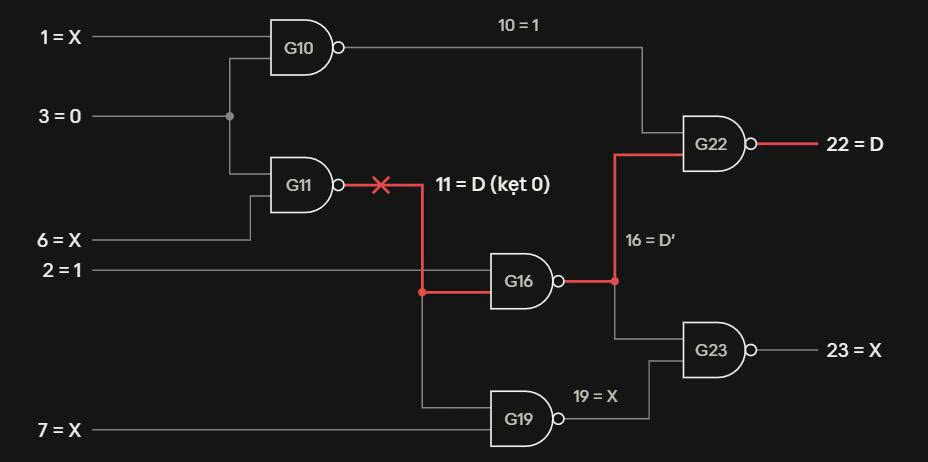
\includegraphics[width=0.72\linewidth]{../report/figures/common/mach_c17.jpg}%
}

\endgroup
\par\smallskip
\small
\begin{tabular}{clcl}
1 & PDCF: $6=0$, $11=D$ & 2 & PDC: $2=1$, $16=\overline D$\\
3 & PDC: $10=1$, $22=D$ & 4 & Justify: $3=0$, $J=\varnothing$
\end{tabular}
\par\smallskip
Cube gốc $(X,1,0,0,X)$; hình sau tổng quát hóa $(X,1,0,X,X)$.
\par
\footnotesize $X=0$: $01000$; PO tốt $(1,1)$, lỗi $(0,0)$.
4 lần chọn cube, 0 backtrack.
\end{frame}

\begin{frame}{PODEM tìm vector bằng quyết định tại PI}
\begin{itemize}
\item Objective xác định net và giá trị cần đạt.
\item Backtrace đưa mục tiêu về một PI chưa gán.
\item Imply mô phỏng tiến, kiểm tra lỗi tại PO.
\item Nhánh thất bại: đảo PI; hết cả hai nhánh: quay về mức cha.
\end{itemize}
\begin{block}{Khác với D-algorithm}
PODEM chỉ quyết định tại PI; net nội bộ được suy ra qua mô phỏng. Vẫn cần tìm kiếm và có thể gặp độ phức tạp hàm mũ.
\end{block}
\small Nguồn: Goel (1981); Wang, Wu và Wen (2006), mục 4.4.4.
\end{frame}

\begin{frame}{c17: hai quyết định phát hiện 11/SA0}
\begin{center}
\begin{tabular}{ccll}
\hline
Bước & Objective & Gán PI & Kết quả chính\\\hline
1 & $(11,1)$ & $3=0$ & $11=D$, $10=1$\\
2 & $(2,1)$ & $2=1$ & $16=\overline D$, $22=D$\\\hline
\end{tabular}
\end{center}
\begin{block}{Kết quả theo thứ tự PI $(1,2,3,6,7)$}
Pattern $X10XX$; 0 backtrack. Điền X bằng 0: $01000$.
\end{block}
\begin{itemize}
\item Cả 8 cách điền X đều phát hiện lỗi tại PO22.
\item Frontier cuối vẫn là $\{19,23\}$; có $D$ tại PO là đủ dừng.
\end{itemize}
\end{frame}

\begin{frame}{Một lần quay lui dẫn tới vector 01}
\[
t=a+b,\quad n=\overline a,\quad out=t\cdot n;\qquad t/SA0.
\]
\begin{enumerate}
\item Thử $a=1$: $t=D$, nhưng $n=0$ làm $out=0$.
\item Đảo $a=0$: $n=1$, $t=X$; tiếp tục kích hoạt.
\item Gán $b=1$: $t=D$, $out=D$; phát hiện lỗi.
\end{enumerate}
\begin{block}{Điểm kiểm tra code P5}
3 hàng gán/đảo, 1 backtrack; pattern $(a,b)=01$. Giới hạn 0 phải trả ABORTED, không phải UNTESTABLE.
\end{block}
\small P2: 4 lần chọn cube, 0 backtrack; P3: 2 phép gán PI trên c17.
Khác đơn vị đếm, chưa suy ra tốc độ. Chờ trace P5 và simulator P6.
\end{frame}

\begin{frame}{P4 -- Vì sao ATPG tuần tự khó?}
\small
\begin{itemize}
  \item DFF lưu trạng thái: $Q(t+1)=D(t)$; $Q(0)$ có thể chưa biết.
  \item Không scan: khó điều khiển $Q$, khó quan sát $D$; cần chuỗi PI
        qua nhiều chu kỳ để khởi tạo, kích hoạt và lan truyền lỗi.
  \item Mạch ví dụ P4: 2 PI, 1 PO, 6 cổng tổ hợp, 1 DFF.
\end{itemize}
\vspace{1mm}
\centering
\resizebox{0.7\textwidth}{!}{\begin{tikzpicture}[>=Latex, node distance=13mm, font=\small]
  \node[draw, rounded corners, minimum width=36mm, minimum height=18mm, align=center] (logic) {Logic tổ hợp\\$N_1,N_2,N_3,D,N_4,Y$};
  \node[draw, rectangle, right=30mm of logic, minimum width=16mm, minimum height=16mm, align=center] (ff) {DFF\\$Q$};
  \draw[->] ([xshift=-18mm,yshift=5mm]logic.west) node[left] {$A$} -- ([yshift=5mm]logic.west);
  \draw[->] ([xshift=-18mm,yshift=-5mm]logic.west) node[left] {$B$} -- ([yshift=-5mm]logic.west);
  \draw[->] ([yshift=5mm]logic.east) -- node[above] {$D$} ([yshift=5mm]ff.west);
  \draw[->] ([yshift=-5mm]logic.east) -- ++(15mm,0) node[right] {$Y$};
  \draw[->] (ff.north) -- ++(0,10mm) -| node[pos=.25,above] {$Q$} (logic.north);
\end{tikzpicture}
}
\end{frame}

\begin{frame}{P4 -- Trải khung và ví dụ $N_3/SA0$}
\small
\begin{itemize}
  \item Thay DFF bằng ràng buộc $Q_{t+1}=D_t$; cùng một lỗi hiện diện
        tại mỗi khung của mạch đã trải.
  \item Dùng hai khung: $(A_0,B_0)=(1,0)$, $(A_1,B_1)=(1,0)$.
\end{itemize}
\begin{center}
\begin{tabular}{@{}c c c c@{}}
\toprule
Khung & $N_3$ tốt/lỗi & $D$ tốt/lỗi & $Y$ tốt/lỗi\\
\midrule
0 & $1/0$ & $0/1$ & $Q_0/Q_0$\\
1 & $1/0$ & $0/1$ & $0/1$\\
\bottomrule
\end{tabular}
\end{center}
\centering Lỗi quan sát tại PO ở khung 1, với cả $Q_0=0$ và $Q_0=1$.
\end{frame}

\begin{frame}{P4 -- Full scan và kết quả kiểm chứng}
\small
\begin{itemize}
  \item Scan FF: shift in $Q$ $\rightarrow$ capture $D$ $\rightarrow$ shift out.
        ATPG tổ hợp xem $Q$ là pseudo-PI, $D$ là pseudo-PO.
  \item Với $N_3/SA0$: $A=1,B=0,Q=0$ cho $D=0/1$.
\end{itemize}
\begin{center}
\begin{tabular}{@{}lcc@{}}
\toprule
Mô hình & Fault universe & Phát hiện\\
\midrule
Full scan, bộ vector vét cạn & 18 stem SA & 18/18\\
Không scan, tối đa 4 khung & 18 stem SA & 18/18 (tối đa 3 khung)\\
\bottomrule
\end{tabular}
\end{center}
\footnotesize Số liệu từ vét cạn và mô phỏng độc lập trên mạch nhỏ;
chưa phải kết quả chạy PODEM của P5/P6.
\end{frame}

\begin{frame}{P5 -- Cài đặt PODEM}

\begin{itemize}
    \item Triển khai PODEM trên logic 5 giá trị.
    \item Các bước chính:
    \begin{itemize}
        \item Imply
        \item Objective
        \item Backtrace
        \item Gán PI
        \item Backtrack
    \end{itemize}
    \item Sử dụng D-frontier để lan truyền fault.
\end{itemize}

\end{frame}

\begin{frame}{Cơ chế tìm kiếm và Backtrack}

\[
\text{Objective}
\rightarrow
\text{Backtrace}
\rightarrow
\text{PI Assignment}
\rightarrow
\text{Imply}
\]

\begin{itemize}
    \item Thử nhánh đầu tiên.
    \item Khi nhánh thất bại, đảo quyết định PI.
    \item Tiếp tục tìm kiếm với decision stack.
    \item Phân biệt \texttt{UNTESTABLE} và \texttt{ABORTED}.
\end{itemize}

\end{frame}

\begin{frame}{Kết quả P5}

\begin{table}
\centering
\begin{tabular}{lccc}
\hline
Fault & Pattern & Backtracks & Status \\
\hline
c17: 11/SA0 & X10XX & 0 & DETECTED \\
Backtrack: t/SA0 & 01 & 1 & DETECTED \\
\hline
\end{tabular}
\end{table}

\vspace{3mm}

\[
\boxed{194\ \text{tests passed}}
\]

\end{frame}
\begin{frame}{P6 -- Kiểm chứng độc lập}
\small
\begin{itemize}
  \item Trình đọc \texttt{.bench} $\rightarrow$ fault list $\rightarrow$ bộ mô phỏng
        lỗi $\rightarrow$ coverage; chỉ dùng thư viện chuẩn Python.
  \item c17: 34 lỗi (22 stem + 12 nhánh), sau gộp tương đương còn 22.
  \item Mọi pattern được mô phỏng lại ở mạch tốt và mạch lỗi: phát hiện nếu
        có PO khác nhau; $X$ điền $0$.
  \item Pattern có $X$ chỉ được xác nhận khi đã vét cạn mọi cách điền $X$.
  \item Mạch tuần tự: $Q@0$ chưa biết; chỉ chuỗi bảo đảm với mọi trạng thái
        đầu mới tính là phát hiện.
\end{itemize}
\end{frame}

\begin{frame}{P6 -- Kết quả c17 và mạch tuần tự}
\small
\begin{center}
\begin{tabular}{@{}lcc@{}}
\toprule
c17, PODEM & Sau gộp & Không gộp\\
\midrule
Fault coverage & 22/22 & 34/34\\
Backtrack trung bình & 0 & 0\\
Pattern trước / sau nén & 22 / 6 & 34 / 7\\
Pattern kiểm chứng sai & 0 & 0\\
\bottomrule
\end{tabular}

\vspace{2mm}
\begin{tabular}{@{}cccc@{}}
\toprule
\texttt{seq\_example}, 18 lỗi & $k=1$ & $k=2$ & $k=3$\\
\midrule
Phát hiện bảo đảm & 1/18 & 13/18 & 18/18\\
\bottomrule
\end{tabular}
\end{center}
\footnotesize Mọi pattern PODEM được fault simulation xác nhận; kết quả tuần tự khớp vét cạn độc lập của P4.
\end{frame}

\begin{frame}{P6 -- Demo và hỏi đáp}
\small
\begin{itemize}
  \item Một lỗi có trace: \texttt{python -m atpg.run circuits/c17.bench --fault 11 0 --trace}
  \item Toàn bộ lỗi: \texttt{python -m atpg.run circuits/c17.bench --all}
  \item Mạch tuần tự: \texttt{python -m atpg.run circuits/seq\_example.bench --unroll 2 --all}
  \item Kiểm thử: \texttt{python -m pytest -q}
\end{itemize}
\vspace{4mm}
\centering {\large Cảm ơn thầy và các bạn đã lắng nghe. Xin mời đặt câu hỏi.}
\end{frame}

\end{document}
